\documentclass[../main]{subfiles}
\begin{document}
\section{Antecedentes Históricos}\label{sec:antecedentes}
        \begin{margintable}\vspace{.8in}\footnotesize
		\begin{tabularx}{\marginparwidth}{|X}
		%Section~\ref{sec:motivation}. Motivation\\
		Section~\ref{sec:antecedentes}. Antecedentes Históricos\\
        Section~\ref{sec:galileo}. Relatividad de Galileo\\
        Section~\ref{sec:postulados}. Postulados de la relatividad especial
		%Section~\ref{sec:license}. Margins\\
		\end{tabularx}
	\end{margintable}
 
        \lipsum[1]
        
        \begin{adjustwidth}{0pt}{-100pt}
          
        \section{Relatividad de Galileo}\label{sec:galileo}   
        
            A finales del siglo XIX, la mecánica clásica era una teoría cuyas ecuaciones de movimiento eran invariantes a las llamadas transformaciones de Galileo. Estas incluyen rotaciones en el espacio 3-dimensional y ``boosts''. Primero repasemos sobre los axiomas de Newton:
            \begin{enumerate}
                \item Existe un marco (sistema) inercial de referencia en el que el movimiento en el cual no se involucran fuerzas externas de una partícula se describe mediante una velocidad constante,
                \begin{equation}
                    \vec{v}=\mathbf{v}=\mathrm{cte}
                \end{equation}
                \item En marcos inerciales, el movimiento de una partícula bajo la influencia de una fuerza se describe mediante la ecuación de movimiento,
                \begin{equation}
                    m \mathbf{a}=\sum_i \mathbf{F}_i=\dot{\mathbf{p}}, \ \mathrm{donde} \ \mathbf{p}=m\mathbf{v}
                \end{equation}
                \item Para cada fuerza con la que una partícula (1) actúa sobre otra partícula (2) existe una fuerza de reacción igual y opuesta con la que la partícula (2) actúa sobre la partícula (1):
                \begin{equation}
                    \mathbf{F}_{(1)\rightarrow (2)}=-\mathbf{F}_{(2)\rightarrow (1)}
                \end{equation}
            \end{enumerate}
        
            Consideremos dos observadores $S$ y $S'$ en movimiento relativo tal como se muestra en la figura \ref{fig:fig1}. Supongamos que ambos sistemas son inerciales, es decir que satisfacen el primer axioma de Newton.

            \begin{figure}[H]
            \begin{adjustwidth}{0pt}{-100pt}
                \centering
                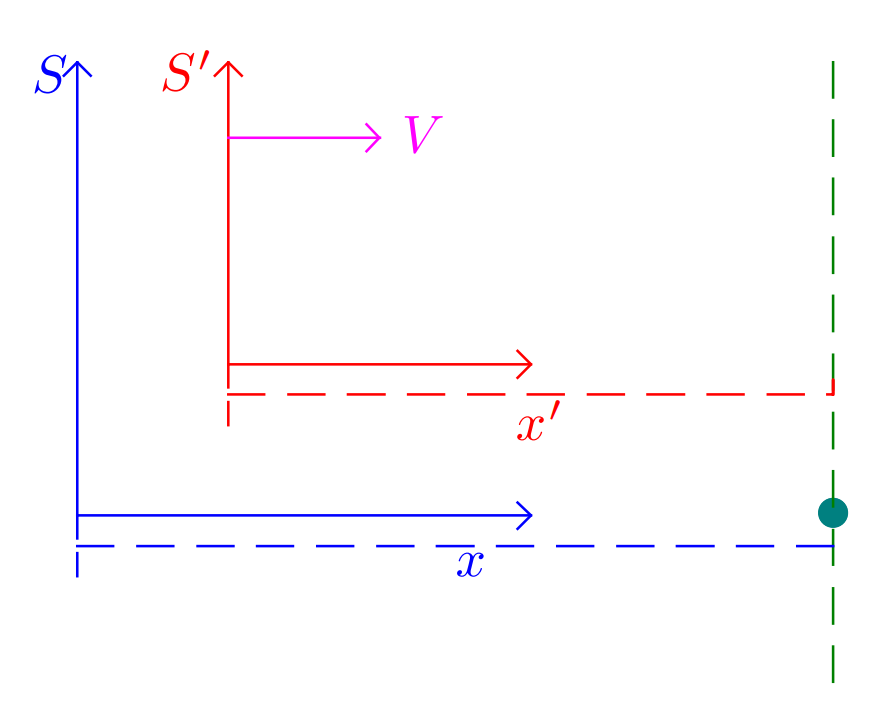
\includegraphics[width=0.7\textwidth]{Física_Moderna/Relatividad especial/fig/RE1.PNG}
                \caption{Dos sistemas de referencia ($S$ y $S'$) en movimiento relativo y un objeto (disco verde) en reposo en relación a $S$.}
                \label{fig:fig1}
            \end{adjustwidth}
            \end{figure}

            Nos colocaremos en una posición tal que para nosotros $S$ este en reposo y $S$ se mueva hacia la derecha con una rapidez $V$ que es constante. Ahora supongamos que hacia una distancia $x$ y hacia la derecha del origen de $S$ hay un cierto objeto (en este caso un disco verde) en reposo con respecto a $S$. La posición del objeto en relación a $S'$ es $x'$. Y nos damos cuenta que la relación entre $x$ y $x'$ será:
            \begin{equation}
                x'=x-Vt
            \end{equation}
            donde $t$ es el tiempo.

            Una suposición subyacente a la construcción de la mecánica Newtoniana es que el tiempo transcurre igual para todos los observadores. Entonces esta transformación de coordenadas puede generalizarse a:
            \begin{equation}
                \begin{aligned}
                    \mathbf{r}'(t')&=\mathbf{r}(t)-\mathbf{V}t \\
                    t'&=t
                \end{aligned}
            \end{equation}

            Estas leyes de transformación constituyen las llamadas \textcolor{red}{transformaciones de Galileo}. Y notamos que la mecánica clásica es invariante bajo estas transformaciones. 
            
            Como el tiempo es el mismo para ambos sistemas de referencia, podemos derivar la posición con respecto al tiempo y obtener:
            \begin{equation}
                \mathbf{v}'=\mathbf{v}-\mathbf{V}
            \end{equation}
            donde $\mathbf{v}$ y $\mathbf{v}'$ son las velocidades del objeto medidas en $S$ y $S'$ respectivamente.

            Derivando nuevamente y considerando que $\mathbf{V}$ es constante, obtenemos:
            \begin{equation}
                \mathbf{a}'=\mathbf{a}
            \end{equation}
            donde $\mathbf{a}$ y $\mathbf{a}'$ son las aceleraciones medidas en $S$ y $S'$ respectivamente.

            Como la fuerza es proporcional a la aceleración, vemos que las fuerzas son invariantes bajo las transformaciones de Galileo.

        \section{Postulados de la Relatividad}\label{sec:postulados}
            Albert Einstein, propuso lo que vendria a ser la Teoría de la Relatividad Especial. Su enfoque se basaba en dos postulados:
            \begin{enumerate}
                \item \textcolor{blue}{Las leyes de la física deben ser las mismas en todos los sistemas de referencia inerciales.}
                \item \textcolor{blue}{La luz se propaga a la misma velocidad $c$ en todos los sistemas de referencia inerciales, sin importar el estado de movimiento del emisor.}
            \end{enumerate}
        \end{adjustwidth}
\end{document}